
\documentclass[12pt, sn-apa,pdflatex,letterpaper]{sn-jnl}

%%%% Standard Packages
%%<additional latex packages if required can be included here>

\usepackage[T1]{fontenc}
\usepackage{tgbonum}
\usepackage{graphicx}%
\usepackage{multirow}%
\usepackage{amsmath,amssymb,amsfonts}%
\usepackage{amsthm}%
\usepackage{mathrsfs}%
\usepackage[title]{appendix}%
\usepackage{xcolor}%
\usepackage{textcomp}%
\usepackage{manyfoot}%
\usepackage{booktabs}%
\usepackage{algorithm}%
\usepackage{algorithmicx}%
\usepackage{algpseudocode}%
\usepackage{listings}%
\usepackage{natbib}
\usepackage[pass]{geometry}
\usepackage{makecell}

\usepackage{lineno}
\linenumbers

%%%%
\raggedbottom
\providecommand{\tightlist}{%
  \setlength{\itemsep}{0pt}\setlength{\parskip}{0pt}}
\renewcommand{\baselinestretch}{1.5} 

\begin{document}


\title[Arriaga meets Kitagawa]{Arriaga meets Kitagawa. Life expectancy decomposition and population subgroups}

\author*[1,2,3]{\pfx{Dr.} \fnm{Timothy} \sur{Riffe} }\email{\href{mailto:tim.riffe@ehu.eus}{\nolinkurl{tim.riffe@ehu.eus}}}

\author*[1]{ \fnm{Rustam} \sur{Tursun-zade} }

\author*[4]{\pfx{Dr.}  \fnm{Sergi} \sur{Trias Llimós} }



  \affil*[1]{\orgdiv{OPIK, Department of Sociology and Social
Work}, \orgname{University of the Basque Country
(UPV/EHU)}, \orgaddress{\city{Leioa}, \country{Spain}, \postcode{48940}, \state{Bizkaia}, \street{Barrio
Sarriena s/n}}}
  \affil[2]{\orgname{Ikerbasque (Basque Foundation for Science)}}
  \affil[3]{\orgdiv{Laboratory of Population Health}, \orgname{Max
Planck Institute for Demographic Research}}
\affil[4]{ \orgname{Centre for Demographic Studies}}

\doublespacing

\abstract{\textbf{Background}: An Arriaga (1984) decomposition partitions differences in life expectancy into contributions from mortality rate differences in each age. A Kitagawa (1955) decomposition partitions a difference between two weighted means into effects from differences in structure and from differences in each element of the weighted value.

\textbf{Objective:} To propose an analytic method to decompose the difference in life expectancy between two populations, each consisting of like-defined subpopulations. Said decomposition would yield effects for each age within each subpopulation and a marginal effect that accounts for composition differences. We illustrate it by examining the sex gap in life expectancy in Spain using education-specific mortality data.

\textbf{Methods:} Life expectancy differences between like-defined subpopulations can be decomposed using the Arriaga method, or a variant thereof. The results of subgroup-specific decompositions can be weighted together using the value component from a Kitagawa decomposition of total life expectancy, given that subpopulations are blended in the radix age. The composition component of the same Kitagawa decomposition gives the effect of subgroup composition on total life expectancy differences.

\textbf{Results:} Notable properties of the method include: (i) it accommodates any number of subpopulations, (ii) it easily incorporates cause-of-death information, and (iii) composition is considered in the radix age. We apply the method to Spanish cause- and education-specific data. We demonstrate that the proposed analytic method is equivalent to reframing the same problem using the generalized linear integral decomposition method.

\textbf{Conclusions:} This method can further disentangle the effects of mortality and composition differences, helping to explain or clarify paradoxes and secular change. Our analytic decomposition method is more computationally efficient than the linear integral or stepwise replacement decomposition methods. We give both R code and spreadsheet implementations of the method.}

\keywords{Decomposition, Mortality, Cause of death, Population Structure, Mortality Inequalities}



\maketitle

\section*{Introduction}\label{intro}

Population-level differences in life expectancy have been widely analyzed using decomposition methods to understand the impacts of mortality differences in age groups \citep[e.g.,][]{arriaga1984measuring, pollard1988decomposition},  or \citet{kitagawa1955components} to understand better the impact of compositional differences in social strata \citep{kitagawa1977mortality}. It has long been known among demographers that improvements in social welfare have the potential to bring large scale improvements in mortality conditions even net of medical improvements \citep{kitagawa1968education}. However, very few demographers have ventured to account for both age-specific effects and compositional effects at the same time \citep{torres2019contribution, hendi2021immigration, su2023educational, su2024subnational},. Disentangling the compositional effect within a conventional age group decomposition would improve our understanding of life expectancy differences between populations. 

The life expectancy decomposition method proposed by \citet{arriaga1984measuring} separates a change in life expectancy into contributions due to mortality changes at different ages. This technique is designed to be practical in that it is framed in terms of lifetable columns expressed in discrete age groups. Two well-known properties of the method are that mortality changes in different ages do not need to be proportional and that the derived contributions sum exactly to the observed difference in life expectancy. A documented but lesser-known property of this method is its asymmetry: the absolute values of age-specific contributions depend on whether we compare population one with two, or vice versa. This is why the method is described in terms of changes rather than group differences; the direction of time is clear, so we always decompose an earlier period against a later period. Importantly, the method is designed to work with homogeneous populations, meaning a single lifetable represents each population. Let's call this method and the variant of it that we later apply the ``Arriaga method''. The Arriaga method has different extensions available to separate the effects of different causes of death within age groups. We seek to extend this method to account for lifetables that are composed of subpopulations with different mortality.

The decomposition method proposed by \citet{kitagawa1955components} separates differences in a weighted mean into contributions from differences in weights (structure) and the value being weighted. Often, the weighted values are rates, but in our case, the weighted values will be the life expectancies of subgroups. This method is well-known to partition differences owing to ``structure'' and ``value'' components, which sum exactly to the observed difference in weighted means. The individual elements of the value being weighted (in our case, life expectancies) have identifiable effects. It is not well-known that the individual elements of the structure component do not have identifiable effects. Instead, the structure effects should be summed up as a total marginal effect due to composition differences. We refer to this method as the ``Kitagawa'' method.

We propose to treat the problem of life expectancy decomposition by age, where a total life expectancy is calculated as the weighted mean of the expectancies of subpopulations. This is only practical when each population is composed of like-defined subpopulations. For example, we may decompose the life expectancy difference between two countries considering differences in education structure, since life expectancy varies by education level \citep{mackenbach2019determinants, trias2023age}. Or, one might wish to calculate a national life expectancy as the weighted average of its regions at two points in time since regional weightings and inequalities may have changed over time. In such scenarios, a decomposition should yield the contribution to the overall life expectancy difference stemming from rate differences in each age (and potentially causes of death) within each subpopulation while giving the overall effect of compositional differences. We propose a straightforward analytic method to perform such decompositions.

In short, differences in life expectancy between subpopulations can be decomposed using the Arriaga method, one of its variants, or by any other life expectancy decomposition method that is acceptably precise with discrete data \citep{Ponnapalli2005,horiuchi2008decomposition,andreev2002algorithm}. In a second step, the Kitagawa method is then used to rescale group-specific life expectancy decompositions, yielding an extra component telling us the importance of compositional differences. We justify this second-pass rescaling and demonstrate that the results of this procedure align with those of a linear integral reframing of the problem, per \citet{horiuchi2008decomposition}. We then apply these methods to decompose the sex gap between Spanish men and women in remaining life expectancy at age 35, considering differences in composition by education attainment around the same age and considering cause-specific mortality rates.


\section*{Method}\label{method}


\subsection*{Notation}\label{notation}

We use the following variables and scripting, most of which are lifetable columns:

\begin{itemize}
\item{${}_nm_a$} mortality rate in the age interval $[a,a+n)$.

\item{$\ell_a$} lifetable survivorship at exact age $a$.

\item{${}_nL_a$} lifetable person-years lived in the interval $[a,a+n)$.

\item{$T_a$} total lifetable person-years lived beyond age $a$.

\item{$e_a$} remaining life expectancy at exact age $a$.

\item{$\pi_a^s$} the population fraction for subgroup $s$ in age $a$.
\end{itemize}

We use the superscript $s$ to index subpopulations comprising the total population, and the superscript ``$1$'' to typically indicate the population with the lower value of $e_0$, and ``$2$'' for the higher value, such that their difference, $\Delta = e_0^2 - e_0^1$, is always positive. Causes of death may be indicated with a $c$ subscript, i.e. $m_{a,c}$. Throughout the manuscript, we assume single-year age groups and omit age interval (left-side) subscripts ($n$) where they would otherwise be due.


\subsection*{Averaging life expectancy}\label{averaging-life-expectancy}

\citet{vaupel2002life} distinguishes between two major approaches to calculate life expectancy for a total population composed of observed subgroups. The dominant approach is based on averaging the mortality rate in each age by aggregating deaths and exposures over all subpopulations and calculating the rate per equation~\eqref{eq_rates}:

\begin{equation}
\label{eq_rates}
m_a = \frac{\sum_i{D_a^i}}{\sum_i{E_a^i}} = \sum_i \pi_a^i m_a^i \quad \mathrm{,}
\end{equation}

\noindent where $D$ and $E$ stand for deaths and exposures, respectively. This is the standard method used implicitly or explicitly by national statistical offices, the Human Mortality Database \citep{wilmoth2021methods}, or the World Population Prospects \citep{wpp2022mp}, among others. \citet{vaupel2002life} called this approach the \emph{current rates} perspective, which treats a heterogeneous population as a homogeneous one.

A second approach derives independent subgroup-specific lifetables and then weights life expectancies together based on an initial mixing composition to obtain the total life expectancy per equation~\eqref{eq_avg}:

\begin{equation}
\label{eq_avg}
e_0 = \sum_s \pi_0^s \cdot e_0^s \quad \textrm{.}
\end{equation}

\noindent This method aligns with Vaupel's \emph{current conditions} approach, at least to the extent that heterogeneous conditions are accounted for using observed strata. This second approach is commonly applied in multistate models with strata combined according to mixed initial conditions to obtain the total population \citep{caswell2018age, caswell2021healthy}, occasionally also with standard lifetables \citep{gupta1988note, muszynska2022mortality}, or when calculating between-within decompositions of variance or other similar summary measures \citep{seaman2019changing, lifeineq}. If the composition is more favorable in younger than in older ages (for example when younger generations have higher average educational attainment), the life expectancy obtained with \eqref{eq_avg} will be higher than one based on \eqref{eq_rates}. This is the total life expectancy approach that our proposed method is designed to decompose.

\subsection*{Kitagawa decomposition}\label{kitagawa-decomposition}

Equation \eqref{eq_avg} treats the total life expectancy as a weighted average, allowing us to precisely decompose a difference in $e_0$, i.e. where $\Delta = e_0^2 - e_0^1$, using the formulas from \citet{kitagawa1955components}.  We presume that population 2 has the higher life expectancy of the two, such that $\Delta$ is positive. Specifically, equation \eqref{eq_kit_comp} gives an overall effect of differences in composition:

\begin{equation}
\label{eq_kit_comp}
\Delta^{(\pi)} = \sum_s \left(\pi^{s,2}- \pi^{s,1}\right) \cdot \overline{e_0^s}\quad \textrm{,}
\end{equation}
 where 
 \begin{equation}\label{eq:e0mean}
     \overline{e_0^s} = \frac{e_0^{s,1} + e_0^{s,2}}{2} 
 \end{equation}

\noindent This result is widely known. Note that the the composition effect must be summed this way because group-specific composition (structure) effects are not well-identified and therefore cannot be interpreted in isolation. Equation \eqref{eq_kit_e0} gives the subgroup-specific effects of differences in life expectancy:

\begin{equation}
\label{eq_kit_e0}
\Delta^{(e_0^s)} = \left(e_0^{s,2} - e_0^{s,1}\right) \cdot \overline{\pi^s}\quad \textrm{,}
\end{equation}
where $\overline{\pi^s}$ is the average composition, analogous to equation~\eqref{eq:e0mean}, and where the superscripts are consistent with those used to calculate the total difference $\Delta$.

Equation~\eqref{eq_kit_sum} states that the observed difference in total life expectancy is the sum of (i) a single component capturing the effect of compositional change and (ii) a set of components giving the contribution of each subgroup's life expectancy difference to the total life expectancy difference. This second effect could equivalently be called the \textit{rate} effect because each life expectancy is ultimately a function of mortality rates.

\begin{equation}
\label{eq_kit_sum}
\Delta = \Delta^{(\pi)}  + \sum_s \Delta^{(e_0^s)}\textrm{.}
\end{equation}


\subsection*{Symmetrical Arriaga
decomposition}\label{symmetrical-arriaga-decomposition}

The \emph{rate} effect as per \eqref{eq_kit_e0} can be viewed as the \emph{net} effect on total life expectancy differences resulting from the age-specific (potentially also cause-specific) differences between like subgroups, as isolated by various life expectancy decomposition methods. In this setting, the choice of method to derive age-specific effects for subgroup-specific changes in life expectancy is not crucial. The \citet{arriaga1984measuring} decomposition approach is widely favored because it is designed for discrete data, it is analytic (implying computational efficiency), and because decomposition results sum exactly to the observed life expectancy difference. Since our application concerns sex differences rather than changes over time, we consider a \emph{symmetrical} Arriaga decomposition. Since we also include cause-of-death information, we transform the symmetrical decomposition results into an implied sensitivity function. This exercise is repeated for each subgroup to decompose group-specific changes in life expectancy (indicated with the superscript $^s$ on each variable):

\begin{equation}
\label{eq_kit_e0_s}
\Delta^s &= e_0^{s,2} - e_0^{s,1} 
\end{equation}

\noindent In this equation $\Delta^s$ is the subgroup-specific ($s$) difference in life expectancy being decomposed, which is composed of age-specific contributions, $\overrightarrow{\Delta_a^s}$ or $\overleftarrow{\Delta_a^s}$ depending on whether we decompose from population 1 to 2 (forward) or from 2 to 1 (backward). The forward age-specific values $\overrightarrow{\Delta_a^s}$ can be calculated following Arriaga's decomposition method, consistent with \citet{arriaga1984measuring} or the presentation in \citet{preston2000demography}, as outlined in equation \eqref{eq_arriaga1}. We use a lifetable radix of 1, meaning $\ell_0 = 1$, to simplify the formula slightly.

\begin{equation}
\label{eq_arriaga1}
 \overrightarrow{\Delta_a^s} = \begin{cases}\ell_a^{s,1} \cdot \left( \frac{L_a^{s,2}}{\ell_a^{s,2}} - \frac{L_a^{s,1}}{\ell_a^{s,1}}\right)+T_{a+n}^{s,2}\cdot\left(\frac{\ell_a^{s,1}}{\ell_a^{s,2}} - \frac{\ell_{a+n}^{s,1}}{\ell_{a+n}^{s,2}}\right)  & \text{$ \forall a < \omega$}\textrm{,}  \\
  \ell_\omega ^{s,1} \cdot (e_\omega^{s,2} -e_\omega^{s,1} ) & \text{$\forall a = \omega $}\textrm{.}
  \end{cases}
\end{equation}

Equation \eqref{eq_arriaga1} represents the first pass of our symmetrical decomposition, while \eqref{eq_arriaga2} is the second pass, which is identical except for swapping population superscripts.

\begin{equation}
\label{eq_arriaga2}
 \overleftarrow{\Delta_a^s} = \begin{cases}\ell_a^{s,2} \cdot \left( \frac{L_a^{s,1}}{\ell_a^{s,1}} - \frac{L_a^{s,2}}{\ell_a^{s,2}}\right)+T_{a+n}^{s,1}\cdot\left(\frac{\ell_a^{s,2}}{\ell_a^{s,1}} - \frac{\ell_{a+n}^{s,2}}{\ell_{a+n}^{s,1}}\right)  & \text{$ \forall a < \omega$}\textrm{,}  \\
  \ell_\omega ^{s,2} \cdot (e_\omega^{s,1} -e_\omega^{s,2} ) & \text{$\forall a = \omega $}\textrm{.}
  \end{cases}
\end{equation}

Importantly,

\begin{align}
\label{eq_sum2}
 -\Delta^s &= \sum_a \overleftarrow{\Delta_a^s} \\
 &= e_0^1 - e_0^2 \nonumber\textrm{.}
\end{align}

A symmetrical estimate of $\Delta_a^s$ is given by the sign-adjusted average of \eqref{eq_arriaga1} and \eqref{eq_arriaga2} for each age, again with a preference for a positive difference:

\begin{equation}
\label{eq_arriaga3}
\Delta_a^s = \frac{\left(\overrightarrow{\Delta_a^s} -  \overleftarrow{\Delta_a^s}\right)}{2}\textrm{.}
\end{equation}

Repeat the symmetrical Arriaga steps to derive age-specific contributions, $\Delta_a^s$, for each life expectancy difference between like-defined subgroups. To take into account information on causes of death, it is best to derive an ad-hoc all-cause sensitivity function, $s_a^s$, by dividing the decomposition result by the mortality rate difference:

\begin{equation}
\label{eq:arr_sen}
s_a^s = \frac{\Delta_a^s}{m_{a}^{s,2} - m_{a}^{s,1}} \quad\mathrm{,}
\end{equation}

\noindent and then multiply age-cause-specific mortality rate differences into $s_a^s$ to obtain the subgroup-specific decomposition by age and cause per equation~\eqref{eq:arr_mxc}.

\begin{equation}
\label{eq:arr_mxc}
\Delta_{a,c}^s = s_a^s \cdot \left( m_{a,c}^{s,2} - m_{a,c}^{s,1}\right)\textrm{.}
\end{equation}

This way of accounting for causes of death is exactly additive. However, if any all-cause mortality rate difference is close to 0, equation~\eqref{eq:arr_sen} is vulnerable, in which case we advise deriving the sensitivity using a more robust (but less precise) approach \citep{coddecomp}

\subsection*{Rescale Arriaga results}\label{rescale-arriaga-results}

 To obtain the \emph{net} impact of $\Delta_a^s$ (or $\Delta_{a,c}^s$) on overall life expectancy change we rescale using \eqref{eq_rescale} to match the life expectancy components from equation \eqref{eq_kit_e0}.

\begin{equation}
\label{eq_rescale}
\Delta_{a,c}^{s,\text{net}} = \Delta^{e_0^s} \cdot \frac{\Delta_{a,c}^s}{\Delta^s} \quad \mathrm{,}
\end{equation}

With the composition effect from equation~\eqref{eq_kit_comp} ( $\Delta^\pi$) and \eqref{eq_rescale}, we have all elements of the proposed decomposition:

\begin{equation}
\label{eq_full}
\Delta = \Delta^\pi + \sum_s \sum_a \sum_c\Delta_{a,c}^{s,\mathrm{net}}\mathrm{.}
\end{equation}


\subsection*{Application}\label{rescale-arriaga-results}

We use data from \citet{trias2023age} on sex-, age-, education-, and cause-specific death counts for individuals aged 35 and over for the years 2016-21 in Spain, which were obtained by request from the Spanish National Statistics Institute (INE). We use all-cause mortality rates for each education- and sex-specific subpopulation from the same source. Educational attainment information is not recorded on death certificates, but INE adds this variable through multiple data linkages \citet{ine2020asignacion}, including municipal population registers (``Padrón'') and the 2011 census. We redistributed deaths with missing education codes ($<2$\% of deaths) across the four educational groups within age, sex, and cause of death classes, proportional to deaths with non-missing education. We then grouped educational attainment into three categories: Low (primary education or less), Medium (secondary education), and High (tertiary or university education). We grouped causes of death from the original ICD10 4-digit codes into 17 main causes: Infectious (ICD-10 codes: A00-B99), Neoplasms (C00-D48), Blood (D50-D89), Endocrine (E00-E90), Mental (F00-F99), Nervous (G00-G99), Circulatory (00-I99), Respiratory (J00-J99), Digestive (K00-K93), Skin (L00-L99), Musculoskeletal (M00-M99), Genitourinary (N00-N99), Congenital (Q00-Q99), Ill-defined (R00-R94), External (chapters S, T, V, W, X and Y), Other causes (chapters H, O and P), and COVID-19 (U071-U072). Moreover, to separate the pandemic period we combined years into two time periods: 2016-2019 and 2020+. Our main results refer to 2016-2019, whereas extra results for 2020-2021 are given in the materials repository.
We smoothed and graduated the original data from 5-year age groups to single ages using a generalized additive model (GAM), including a P-spline over age and population offsets \citep{mgcv2011,mgcv2017}. The GAM formula is given in equation~\eqref{gam_model}, using the Quasi-Poisson family of models to account for possible overdispersion or Negative Binomial model in cases with a more substantial overdispersion:

\begin{equation}
\label{gam_model}
\log(\mu_a) = \beta_0 + f(a) + ln(pop_a)
\textrm{.}
\end{equation}

\FloatBarrier
\section*{Results}\label{results}
We present empirical results for the decomposition of the sex difference in life expectancy in 2016-2019.
Table 1 presents the components of the Kitagawa decomposition for males and females. In this context,  $\pi$ c represents the educational structure, while $e(35)$ denotes life expectancy at age 35 (``rate'' element in original Kitagawa terms). The table also gives the corresponding education structure and life expectancy differences between sexes. The final element,  $\Delta^{(e_{35}^s)}$, is the decomposition result, which gives the education group contribution.
The largest life expectancy gap is observed among individuals with Primary and Secondary education levels, and this gap is lower for those with Higher education.

\begin{table}[ht]
\centering
\begin{tabular}{l|lccccccc}
  \hline
  Education  & $\pi^f$ & $\pi^m$ & $\pi^f - \pi^m$ & $e(35)^f$ & $e(35)^m$ & $\overline{e(35)}$ & \makecell{$e(35)^f -$\\$ e(35)^m$} & $\Delta^{(e_{35}^s)}$ \\ 
  \hline
   Primary  & 0.09 & 0.10 & -0.01 & 48.21 & 42.47 & 45.34 & 5.74 & 0.54\\   
   Secondary  & 0.41 & 0.52 & -0.11 & 50.29 & 44.52 & 47.40 & 5.78 & 2.69\\ 
   Higher  & 0.50 & 0.38 & 0.12 & 51.30 & 46.92 & 49.11 & 4.38 & 1.92\\   
   \hline \hline
\end{tabular}
\caption{Elements of the Kitagawa decomposition, sex gaps in life expectancy in Spain, 2016-19}
\label{tab:my_table}
\end{table}

The corresponding difference in education-specific life expectancy is also illustrated in Figure 1. This figure additionally shows the differences observed for standard aggregated (non-stationary) versus radix-weighted life expectancy (stationary).

\begin{figure}[ht!]
    \centering
    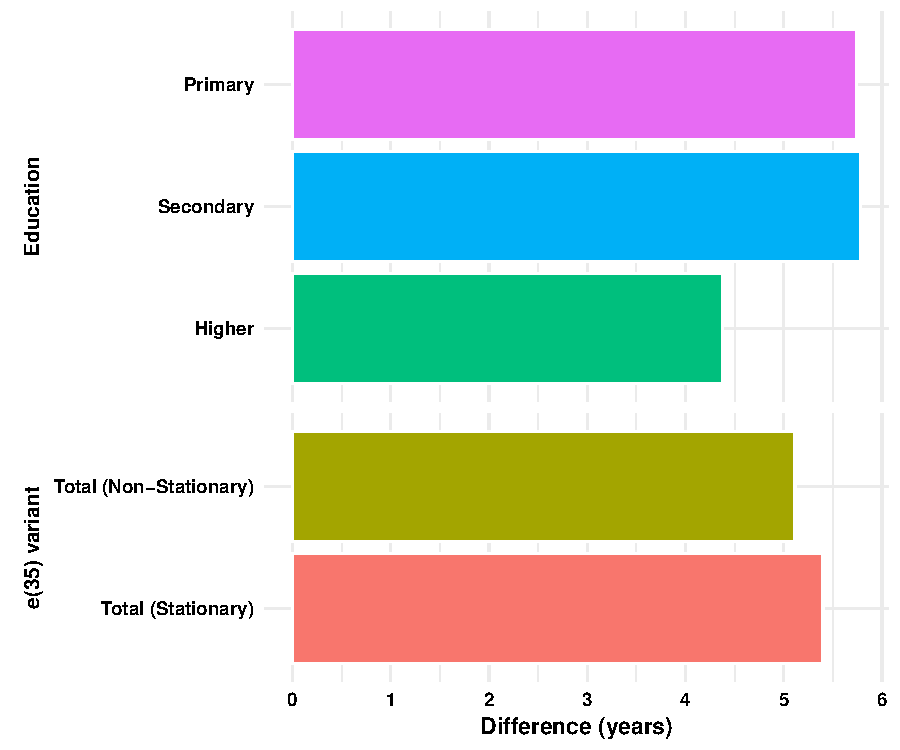
\includegraphics[width=.8\linewidth]{manuscript/fig1.pdf}
    \caption{The Female-Male difference in $e(35)$ by education and population type, Spain 2016-19. }
    \label{fig:enter-label}
\end{figure}
Figure 2 is complementary to Figure 1 and represents the education contribution to the $e(35)$ sex gap with the educational composition component contribution, about 3 months, being added to the figure.

\begin{figure}[ht!]
    \centering
    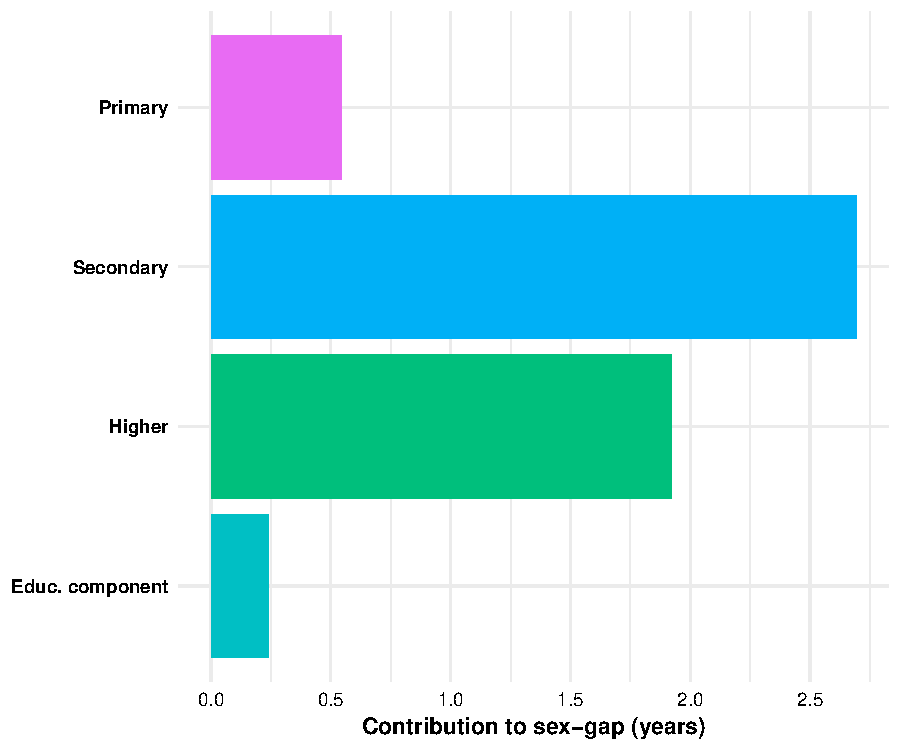
\includegraphics[width=.8\linewidth]{manuscript/fig2.pdf}
    \caption{Education structure contribution to total $e(35)$ sex gap, Spain 2016-19}
    \label{fig:enter-label}
\end{figure}

Figure 3 illustrates the cause-specific contributions to the life expectancy gap. The majority of this gap is explained by differences in mortality from cancer, circulatory diseases, respiratory conditions, and external causes. Neoplasms alone contribute to almost two full years of life expectancy. The only categories where males have a slight advantage in mortality are musculoskeletal and other minor causes. 

\begin{figure}[ht!]
    \centering
    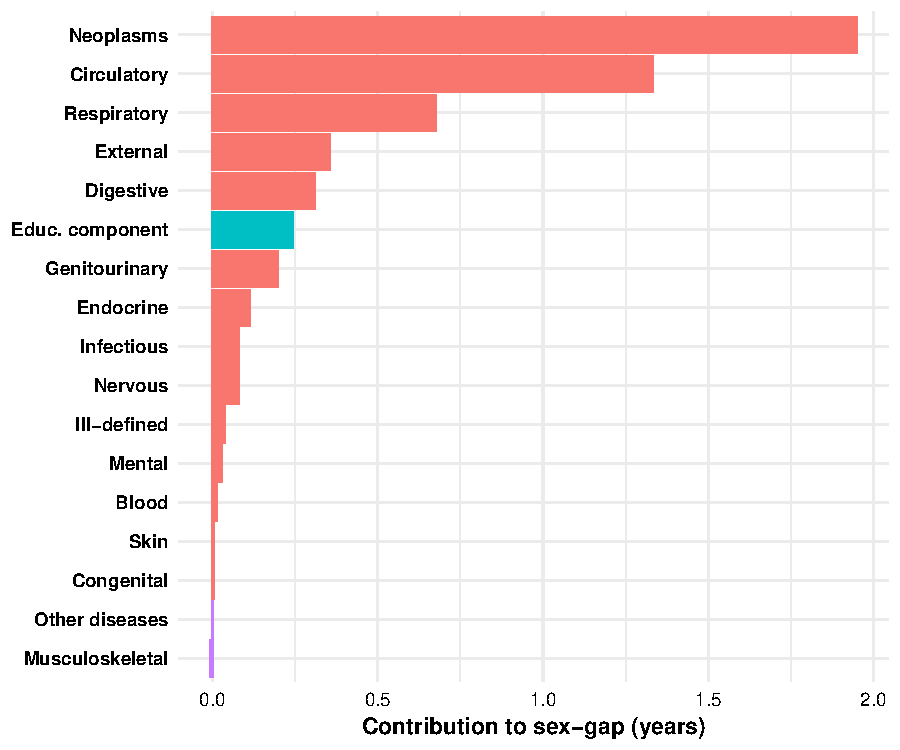
\includegraphics[width=.8\linewidth]{manuscript/fig3.pdf}
    \caption{Cause-specific contribution to sex difference in total $e(35)$, Spain 2016-19. The Education structure contribution is presented in a different colour}
    \label{fig:enter-label}
\end{figure}

Further decomposition of cause-specific differences for age and education components of composed decomposition is shown in Figure 4. The majority of the difference in neoplasm mortality is concentrated in the older age group of 70-80 years. The circulatory component is observed in slightly younger ages and is more uniformly distributed between ages 60 and 80. In contrast, the respiratory component is more pronounced around age 85. The external causes of death primarily contribute to the difference in younger ages and since our data is bounded below by the age of 35, the full effect cannot be fully observed here.

\begin{figure}[ht!]
    \centering
    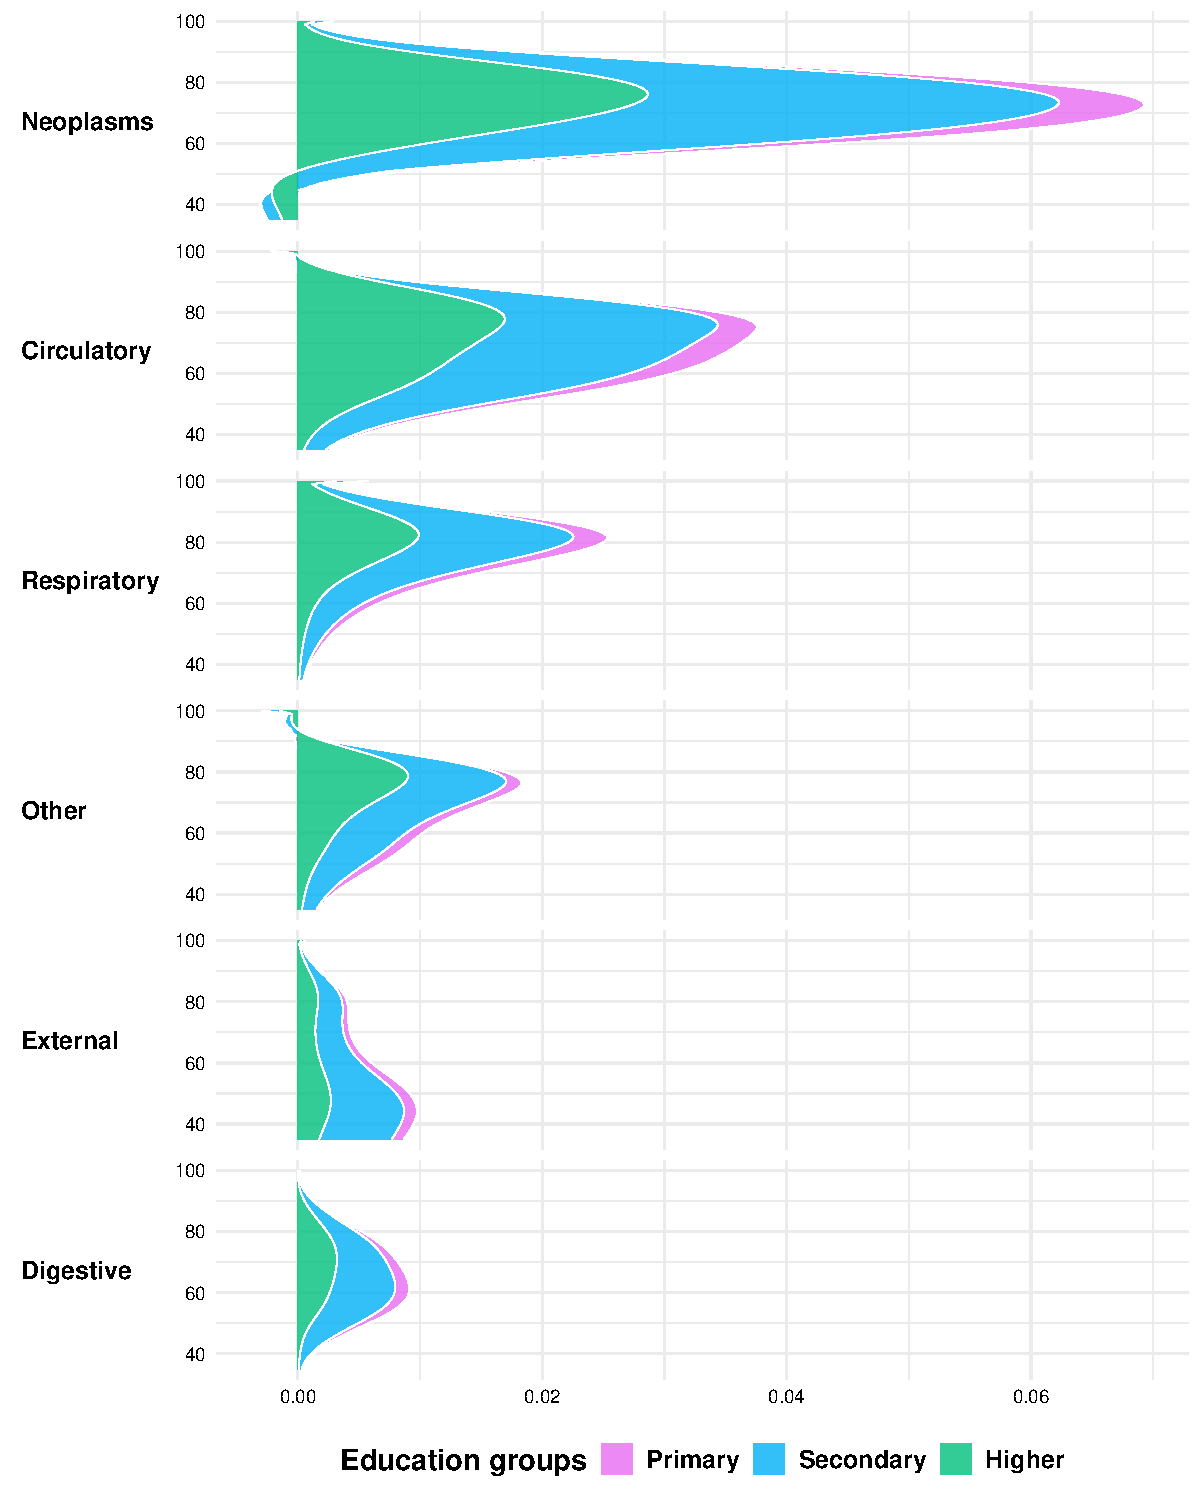
\includegraphics[width=0.8\linewidth]{manuscript/fig4.pdf}
    \caption{The contributions of age, education, and major causes of death to the sex gap in total $e(35)$.}
    \label{fig:enter-label}
\end{figure}

\FloatBarrier

\section*{Discussion}\label{discussion}

In this paper, we propose a method for decomposing the differences in life expectancy that accounts for the compositional effects of education and causes of death between two populations mixed in the radix. Deriving an analytical solution for decomposition offers several advantages over alternative methods, particularly in terms of simplicity, speed, and repeatability. Unlike the linear integral method \citet{horiuchi2008decomposition}, which requires programming expertise, our approach can be executed swiftly and efficiently, even within spreadsheet-like environments. The computational efficiency of our method allows for the calculation of confidence intervals using bootstrapping.

Using the Kitagawa decomposition approach \citep{kitagawa1955components} to weigh together group-specific paired decompositions, our method can be generalized to address many decomposition problems involving structural compositional components, and it is not bound to mortality analyses. However, this post-weighting approach is most suitable for cases where populations are blended in a radix. In contrast, other approaches in the literature  \citep{torres2019contribution,su2023educational,su2024subnational,hendi2021immigration} decompose referring to the standard \emph{current rates} \citep{vaupel2002life} method of calculating life expectancy. These approaches treat the age pattern of group prevalence differently, in essence fixing group prevalence (weights) rather than making prevalence depend on mortality. We point out that mortality is often one of the major drivers of how group prevalence weights change over age.

 When incorporating information on causes of death, a potential vulnerability of our method arises when the difference in mortality rates in the denominator of equation~\eqref{eq:arr_sen} approaches zero (compare with Box 4.3 of \citet{preston2000demography}), rendering an implausible result. In this case, one may prefer to use a direct approximation or numerical estimate of the life expectancy sensitivity in equation~\eqref{eq:arr_mxc}.

Our empirical results indicate that the sex gap in life expectancy remains a significant issue in Spain across all educational strata. However, it is about 25\% lower in the Higher education group. This can be attributed to several factors, including females' lower engagement in risky behaviours \citep{ross2012education,cook2001knowing,byrnes1999gender,kritsotakis2016gender,olson2017gender}, better jobs and greater health awareness of males with higher education \citep{lawrence2017college,ross1995links,ross2012education, mcmahon2009higher}. In terms of causes, neoplasms, circulatory diseases, and respiratory diseases account for the largest contributions to the sex gap. Given that the male disadvantage peaks around ages 65-85 (birth cohorts 1934-1951), this difference can be partly explained by the differences in smoking patterns between males and females within each subpopulation \citep{haeberer2020social}. Since our findings are based on education as a marker of socioeconomic status, they refer only to ages above 35. Therefore, we do not here measure the full power of socioeconomic status or different causes of death in driving the overall sex gap in life expectancy. Further studies could use our method to explain the sex gap using geography, socioeconomic status, and causes of death.

\hypertarget{Conclusion}{%
\section*{Conclusion}\label{conclusion}

Our proposed combination of two analytical decomposition methods can handle the problem of a composed life expectancy, thereby giving an efficient framework for analyzing differences in life expectancy while accounting for population heterogeneity on fixed characteristics. We give both R code and spreadsheet implementations of the method. Our framework is straightforward to use and does not require high computational capacity, making it suitable for implementation in a spreadsheet-like environment while providing results comparable to those of the widely used Horiuchi method. The main advantages of the proposed method are its computational efficiency and ease of implementation over the commonly used Horiuchi method. Further efforts in alleviating the sex gap in mortality are required. The main cause of death contributions suggests that attention to the determinants of neoplasms, cardiovascular, and respiratory diseases could play a substantial role in reducing the sex gap in life expectancy.
 
\bibliography{bibliography.bib}

\backmatter

\bmhead{Supplementary information}

If your article has accompanying supplementary file/s please state so here.

\bmhead{Acknowledgments}

Thanks to Michael Lachanski for posing the question that led to the solution we present here, to Jonas Schoeley for first raising our attention to the composition problem with the Kitagawa method, and to the MPIDR Laboratory of Population Health for posing assorted questions in September 2023 that also led to this work.

\subsection*{Funding}\label{funding}

This work was partly financed by grant nr SR22-00502 from \emph{la Caixa Foundation} and grant number PID2022-142762OA-I00 from the Spanish \emph{Ministerio de Ciencia e Innovation}. STL acknowledges research funding from the Ramon y Cajal program of the same Ministry (RYC2021-033123-I).


\subsection*{Conflict of interest}\label{conflict-of-interest}

The authors declare no conflict of interest


\subsection*{Availability of data and
materials}\label{availability-of-data-and-materials}

We cannot share the original data that this study is based on. We do 


\subsection*{Code availability}\label{code-availability}

All code used here is available in an open \texttt{GitHub} repository
\url{https://github.com/timriffe/arriagakitagawa}
}
\end{document}
